\subsection{Linear regression with forward selection}
In order to obtain the best model with linear regression, we want to avoid overfitting our data. Forward selection is a method to find a set of attributes to minimize the test prediction error, without evaluating models for all subsets of attributes. This method assumes that the attributes are independent, and iteratively adds attributes which result in the lowest prediction error, resulting in a local minimum. When no attribute can lower the prediction error further, the process stops, and a model has been found. The feature selection procedure is as outlined in section 9.2 in the course notes \cite{coursenotes}.

Since our attributes represent relative weight percentage of the elements in the glass, the assumption of independent attributes seem to oversimplify the situation. For instance, adding more K might lower the percentage of Al in the glass. Another factor which might object to the assumption is, if the interaction between the elements in the glass effect the refractive index, e.g. combinations of elements might effect the final structure of the glass.

The model obtained by feature selection can be seen on the left in figure \ref{fig:linreg_fs}. The data has been standardized by subtracting the mean and dividing by the standard deviation. For each selection of a feature, the new feature is evaluated with 10-fold cross validation to hopefully dismiss unwanted bias. On the right in figure \ref{fig:linreg_fs}, we check if the model is enhanced by also adding all binary combinations of the attributes, to see if the interaction between attributes have impact on the refractive index.

\begin{figure}[H]
    \centering
    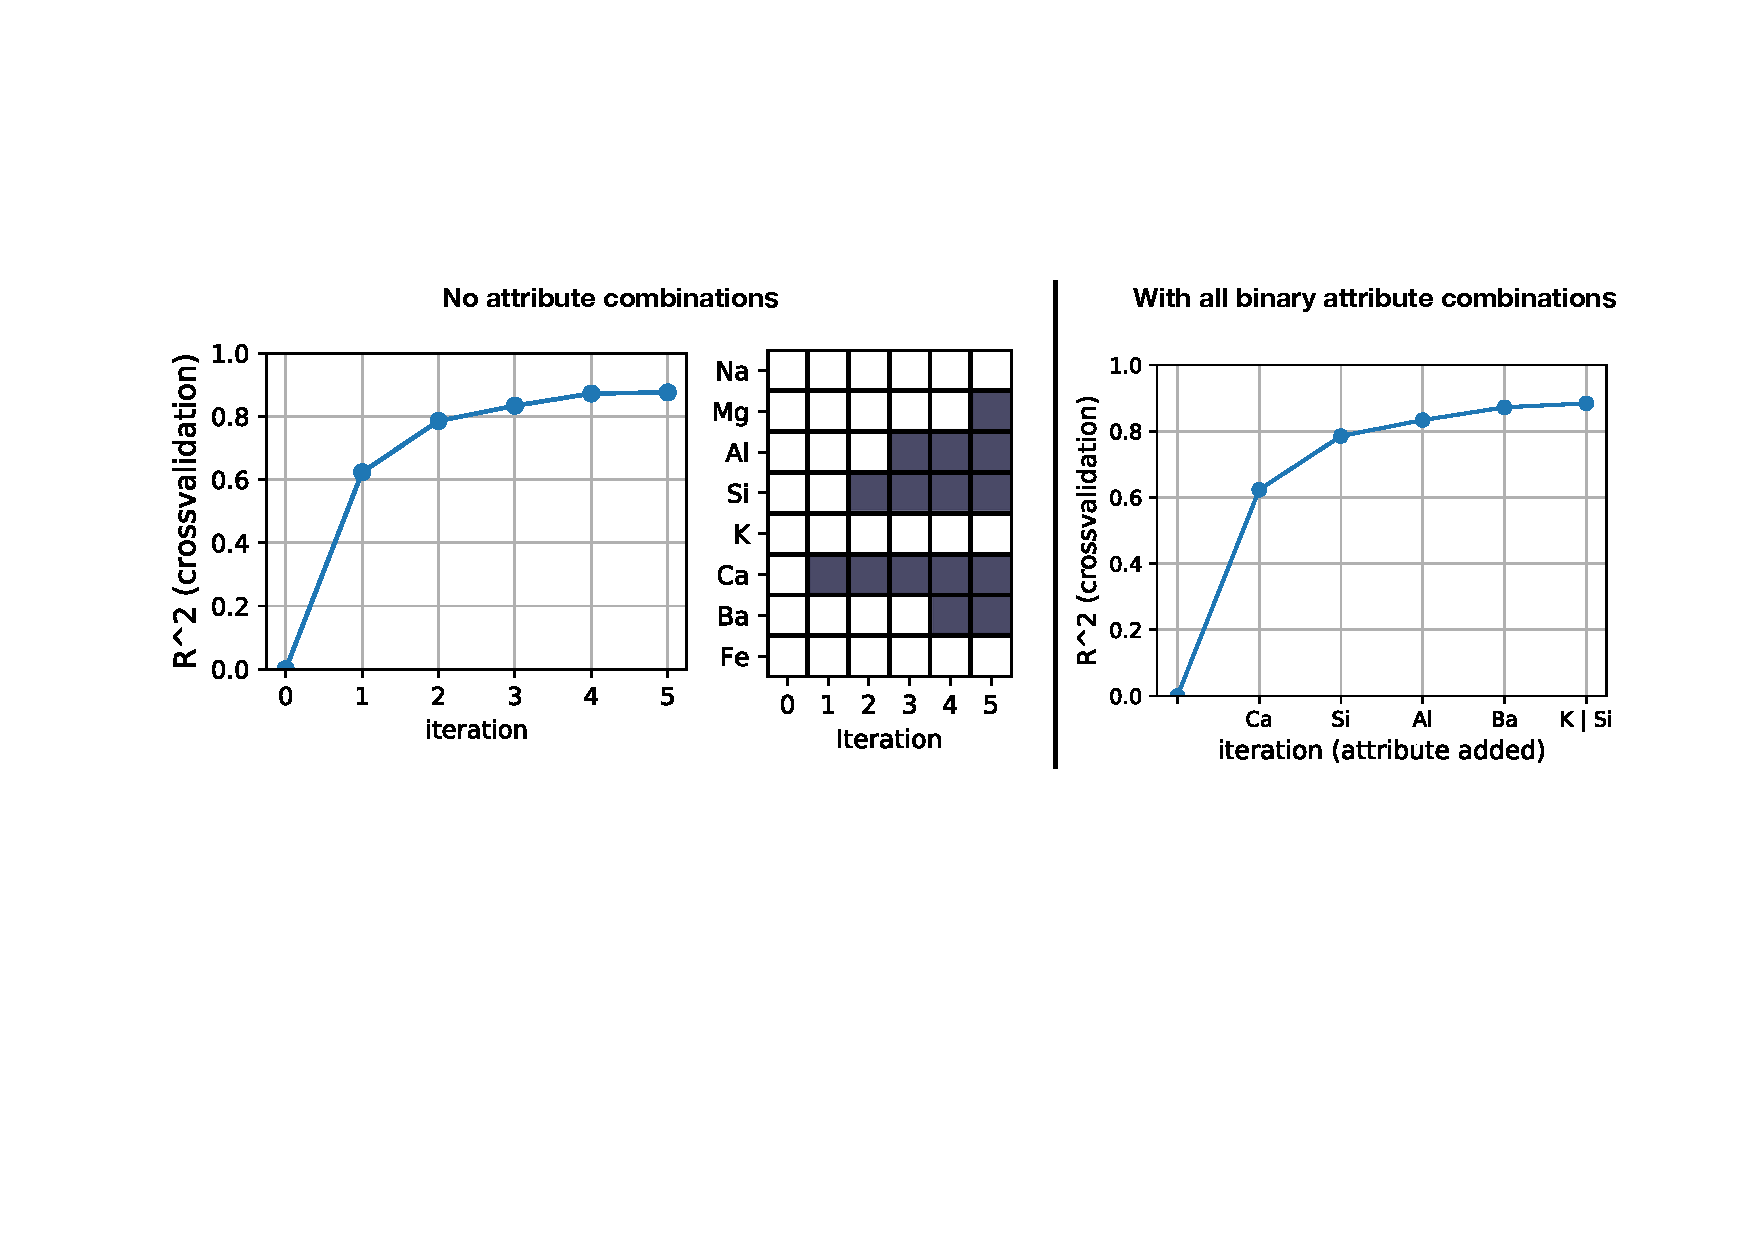
\includegraphics[width=\textwidth]{fig/RegressionPlot.pdf}
    \caption{Linear regression model found by forward feature selection. \textbf{Left side:} Model based on the original set of attributes. Found regression: $\widetilde{\texttt{IR}} = 2.65\cdot 10^{-13} + 0.208 \cdot \texttt{Mg} - 0.229 \cdot \texttt{Al} - 0.312 \cdot \texttt{Si} + 0.808 \cdot \texttt{Ca} + 0.271 \cdot \texttt{Ba}$. Final $\text{R}^2$ value is 0.876. 
    \textbf{Right side:} Model based on original set of attributes and all binary combinations. Found regression: $\widetilde{\texttt{RI}} = 8.93\cdot 10^{-3} - 0.277 \cdot \texttt{Al} - 0.42 \cdot \texttt{Si} + 0.647 \cdot \texttt{Ca} + 0.172 \cdot \texttt{Ba} + 0.046 \cdot \texttt{K}\cdot\texttt{Si}$. Final $\text{R}^2$ value is 0.884.
    The models and plots are guided by \texttt{ex6\_2\_1}.}
    \label{fig:linreg_fs}
\end{figure}

In figure \ref{fig:linreg_fs} the horizontal axes corresponds to each step in the feature selection method, starting from no features to, in this case, 5 features in total. 

The vertical axis for the middle plot represents the different features chosen from, and the dark squares represent the chosen feature set for each iteration, this is not shown for the right plot, since it would contain all $M^2+M \rightarrow 8^2+8 = 72$ features, instead the added features are shown in the iteration ticks. The vertical axis for the remaining two plots represents the $\text{R}^2$ value corresponding to the prediction error of the evolving model for each iteration of the feature selection. The $\text{R}^2$ value is calculated as $1 - \sum_{i} \left(y_i - f_i\right)^2/\sum_{i} \left(y_i - \bar{y}\right)^2$, where $y_i$ is the actual RI of observation $i$, $f_i$ is the model prediction for observation $i$ and $\bar{y}$ is the average RI from the observations. 

To check if the model would benefit from further transformations of the data, we plot the residuals of the model predictions for each of the attributes, and check of any patterns are present. The plots are seen in figure \ref{fig:resPrAtt}.

\begin{figure}[H]
    \centering
    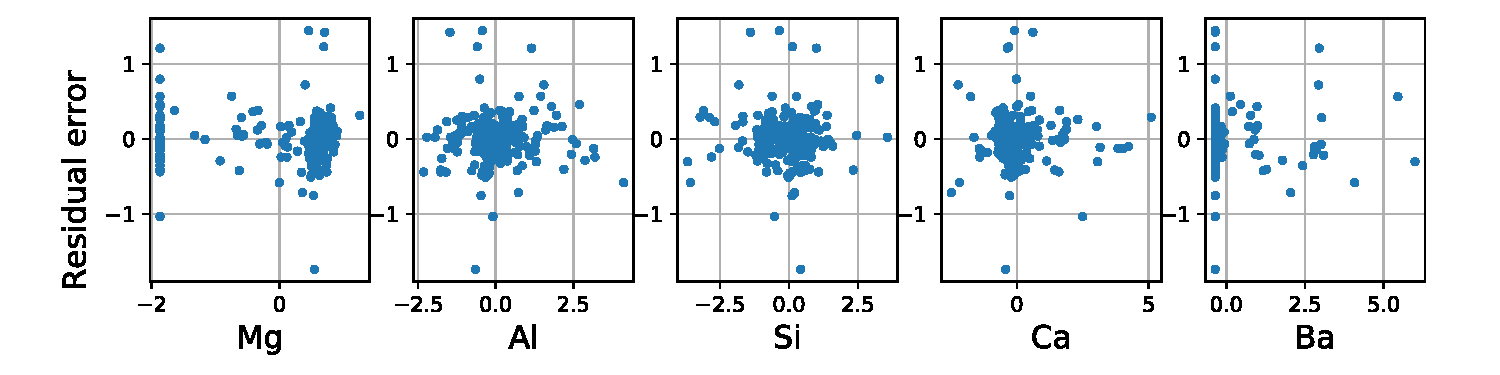
\includegraphics[width=\textwidth]{fig/reg_residuals.pdf}
    \caption{Residuals of RI predictions from the model found by feature selection on the original attribute set. The plot is guided by \texttt{ex6\_2\_1}.}
    \label{fig:resPrAtt}
\end{figure}

Looking at the residuals plotted in figure \ref{fig:resPrAtt} we don't see any apparent patterns. The content of Mg and Ba is little to nothing in many observations, which is seen on the plots as a cluster of residuals with the same low value. Since the data is centered, the observations with low quantities are seen as negative values. Looking at figure \ref{fig:resPrAtt}, no attributes will benefit from a e.g. $\log x$ or $x^2$ transformations, the data will not be further transformed. Likewise, no patterns are found in the residuals for the model including all binary combinations of attributes.

%As earlier mentioned, the combinations of elements might influence the final structure of the glass. To check for this, we run feature selection the original attributes together with all combinations of two elements, to see if we find attribute combinations which contain useful information, resulting in $M^2+M$ possible features. The amount of elements in our glass composition is 8, resulting in $8^2+8=72$ possible features to select from. The model selecting between attribute and possible binary combinations is shown in figure \ref{fig:linreg_fs_combi}.

%\begin{figure}[H]
%    \centering
%    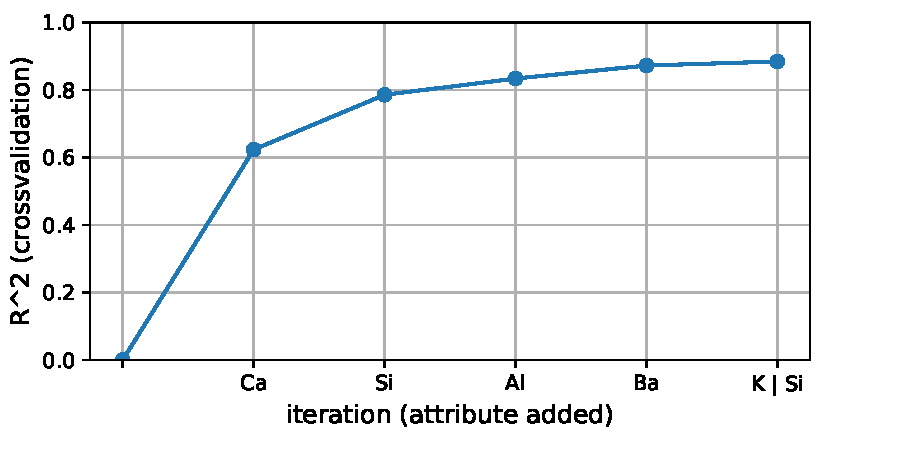
\includegraphics[width=0.7\textwidth]{fig/reg_allCombi_Trans_Mean_Std.pdf}
%    \caption{Linear regression model found by forward selection of attributes and possible binary combinations of attributes. The resulting model predicts the refractive index by the equation: $\widetilde{\texttt{RI}} = 8.93\cdot 10^{-3} - 0.277 \cdot \texttt{Al} - 0.42 \cdot \texttt{Si} + 0.647 \cdot \texttt{Ca} + 0.172 \cdot \texttt{Ba} + 0.046 \cdot \texttt{K}\cdot\texttt{Si}$. Final $\text{R}^2$ value is 0.884. The model and plot are guided by \texttt{ex6\_2\_1}.}
%    \label{fig:linreg_fs_combi}
%\end{figure}

%The feature plot to the right of the error plot in figure \ref{fig:linreg_fs} is not shown in figure \ref{fig:linreg_fs_combi} as it would be a massive 72 row high figure. Instead the feature added in each iteration is displayed on the horizontal axis. Comparing the two models, we see that the first four features are identical. The only difference, is that the combination of K and Si is chosen instead of Mg. As for the previous model, no patterns are found in the residuals, so no further transformations of the data is performed.

Comparing the $\text{R}^2$ values of the two models in figure \ref{fig:linreg_fs}, we see that the model with attribute combinations is slightly better. The difference is from $\text{R}^2 = 0.876$ to $\text{R}^2 = 0.884$. Since only the last chosen feature is changed the difference is expected to be slight, as the impact of the features get progressively smaller each iteration.